%\section{پیاده‌سازی کنترل‌کننده \lr{LQIDG} بر رویه کانال پیچ}\label{roll_lqidg_section}
%در بخش
%\ref{roll_lqidg_section_simulation}
%شبیه‌سازی تک کانال استند چهارپره در حضور کنترل‌کننده \lr{LQIDG} انجام شد. 
در ادامه به پیاده‌سازی کنترل‌کننده \lr{LQIDG} بر رویه کانال پیچ استند سه درجه آزادی پرداخته می‌شود.
در پیاده‌سازی از ضرایب وزنی بهینه به دست آمده در قسمت شبیه‌سازی استفاده شده‌است.
\begin{figure}[H]
	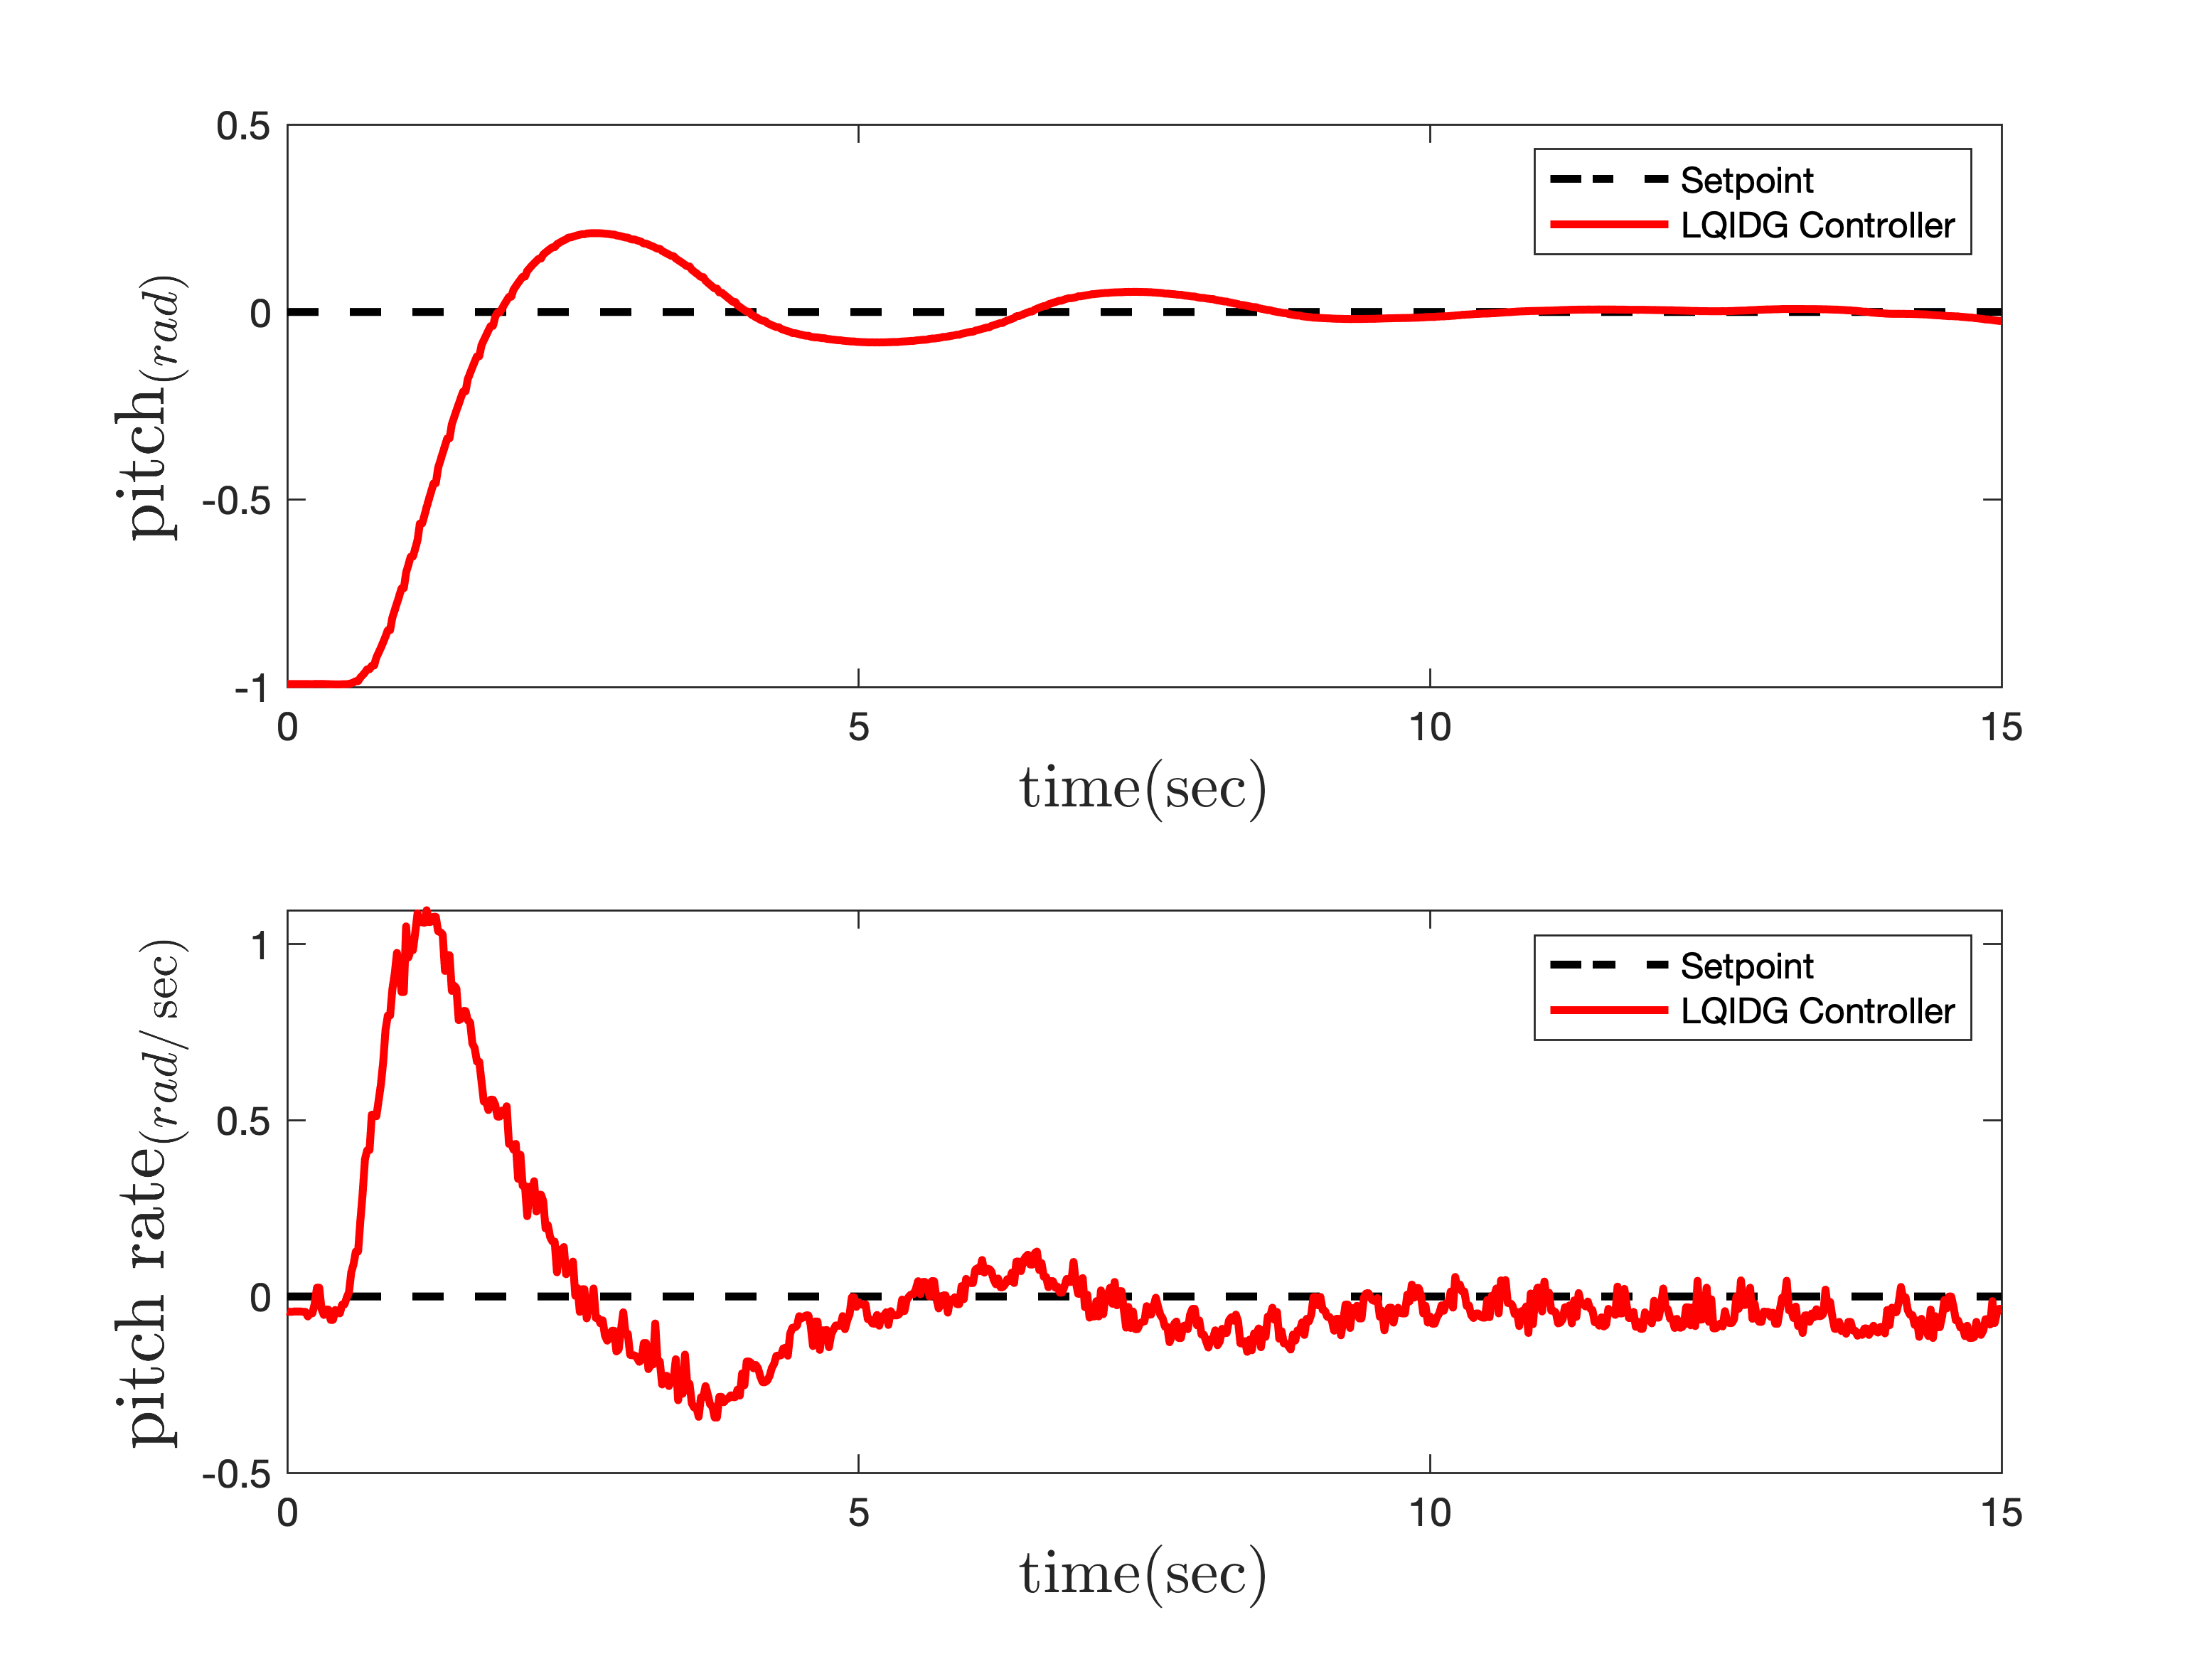
\includegraphics[width=.48\linewidth]{../Figures/Calibration/LQIDG/Pitch/lqidg_pitch.png}
	\centering
	\caption{عملكرد کنترل‌کننده  LQIDG در کنترل زاويه پیچ (تعقیب ورودی صفر)}
\end{figure}

%\begin{figure}
%	[width=12cm]
%	\centering
%	\begin{subfigure}
%		\centering
%		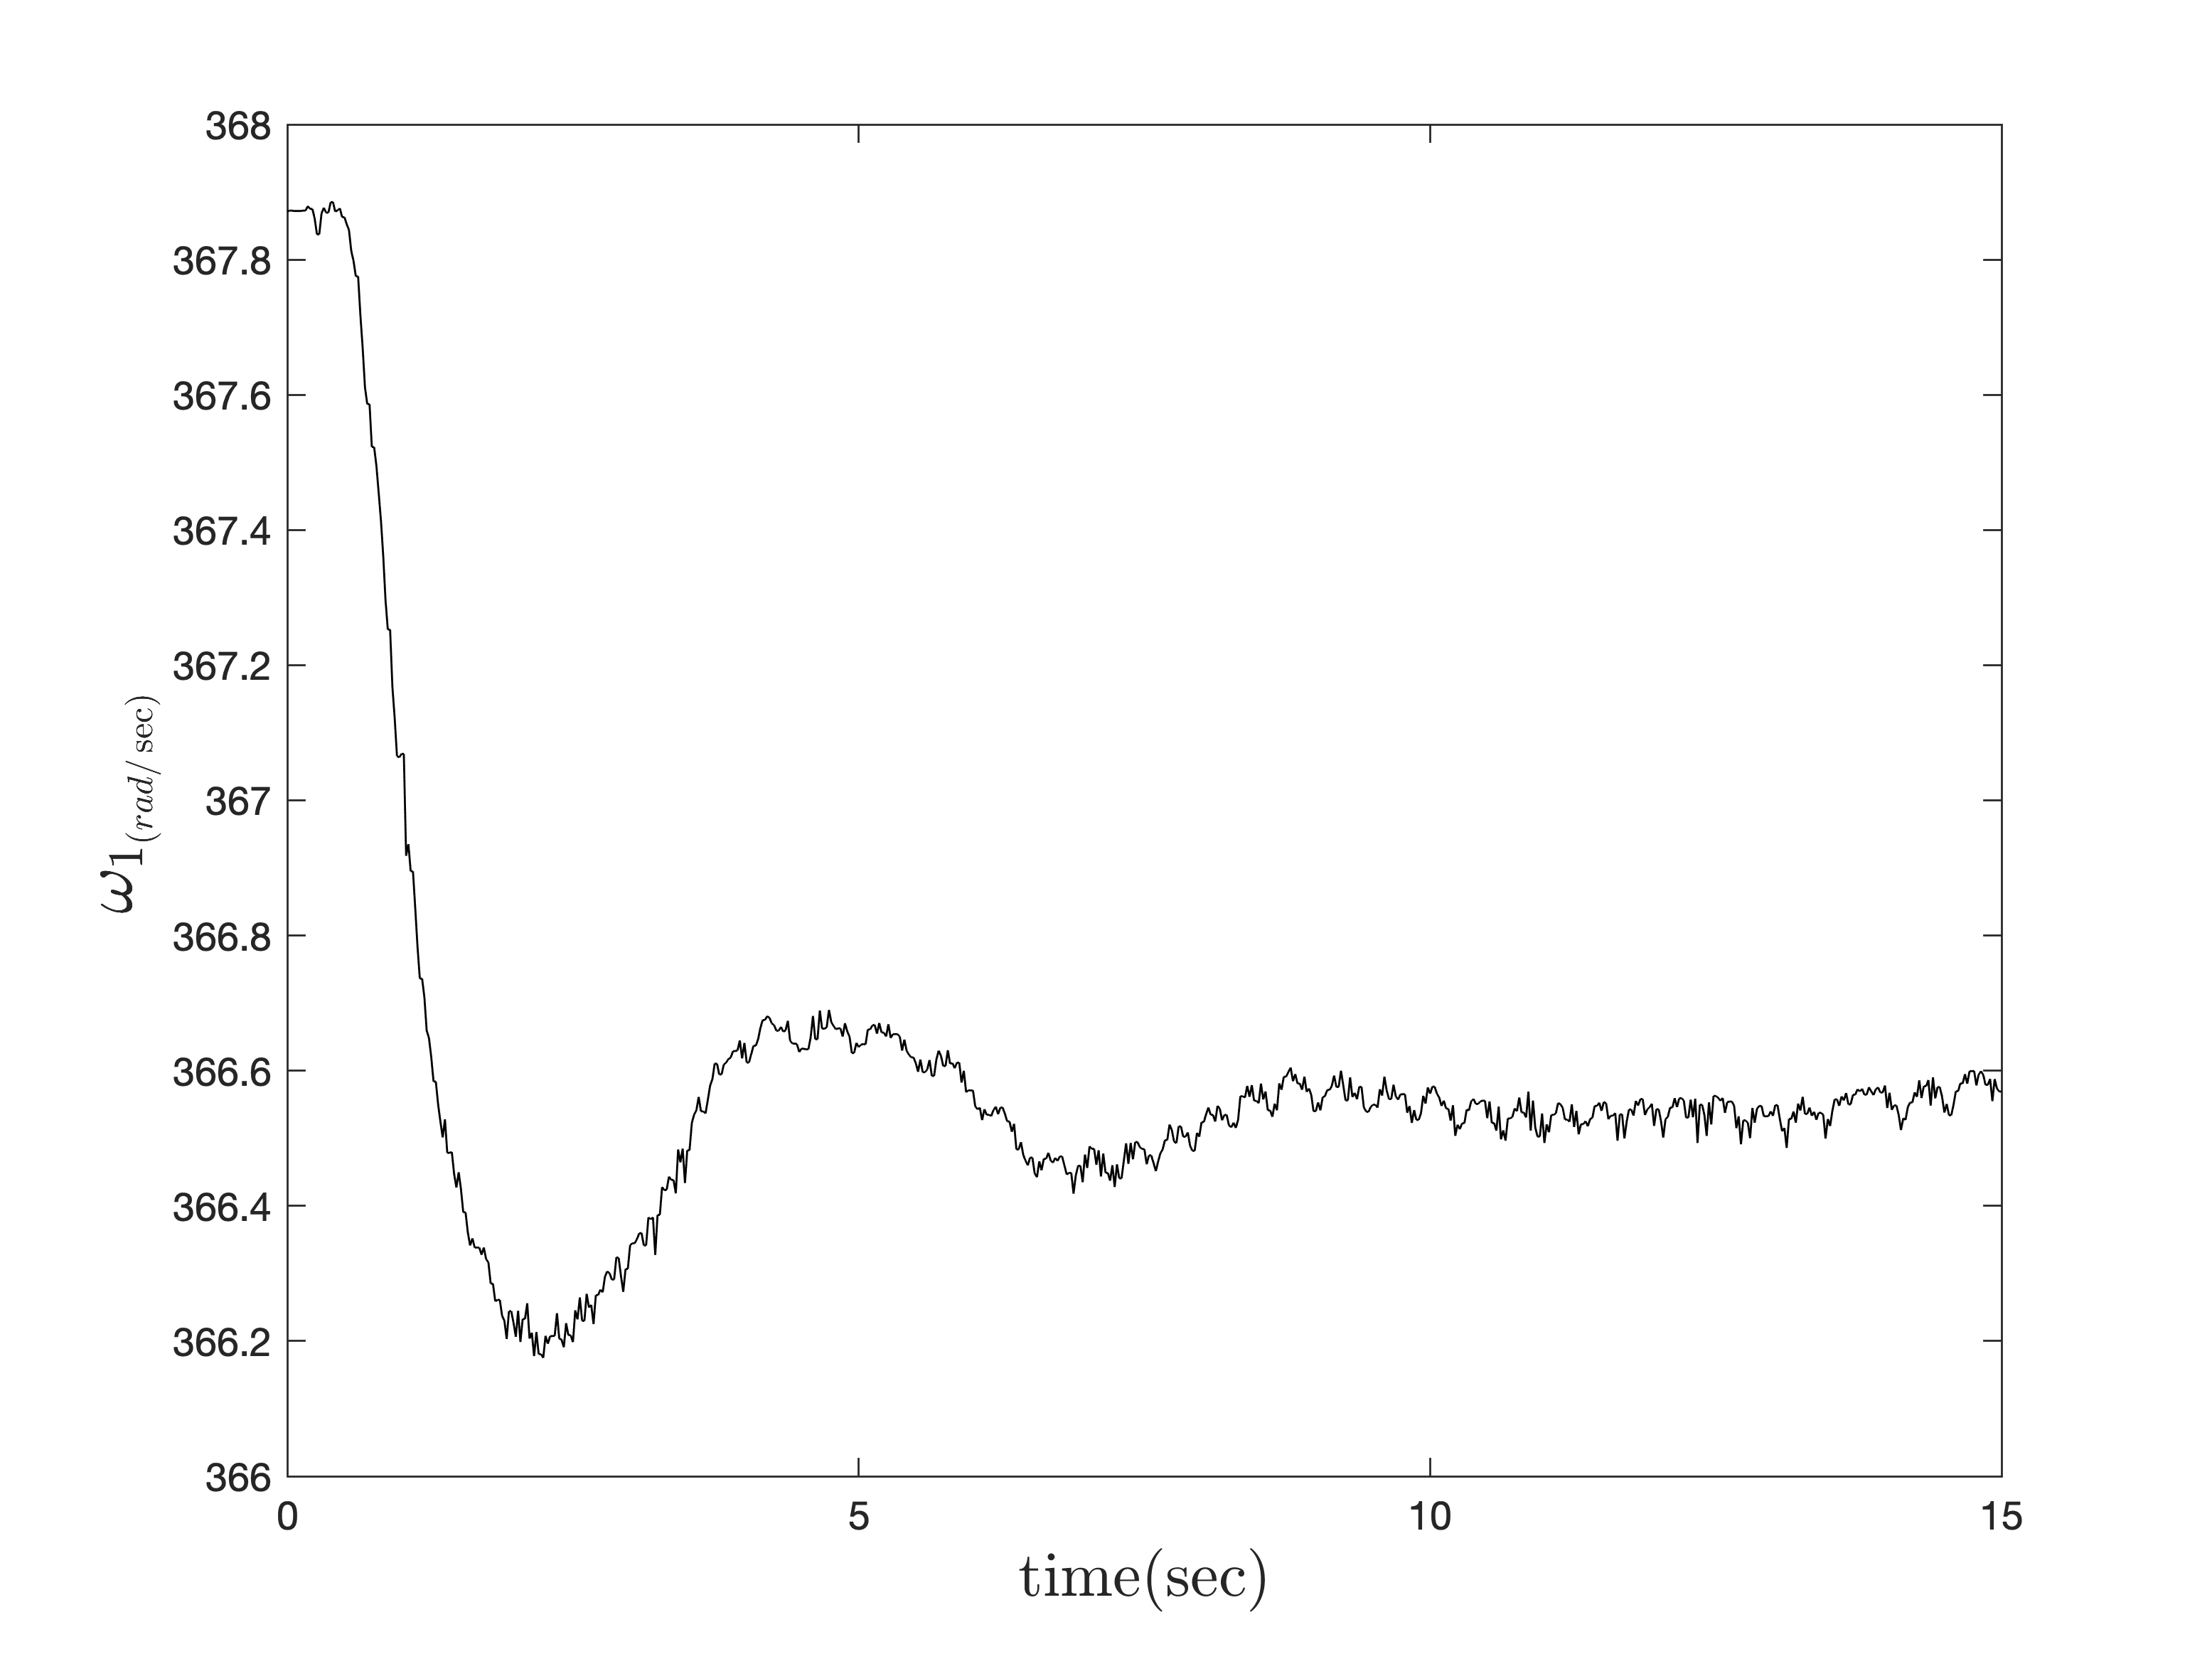
\includegraphics[width=12cm]{../Figures/Calibration/LQIDG/Pitch/lqidg_Omega_1.png}
%		\caption{موتور شماره یک}
%	\end{subfigure}
%	\begin{subfigure}
%		\centering
%		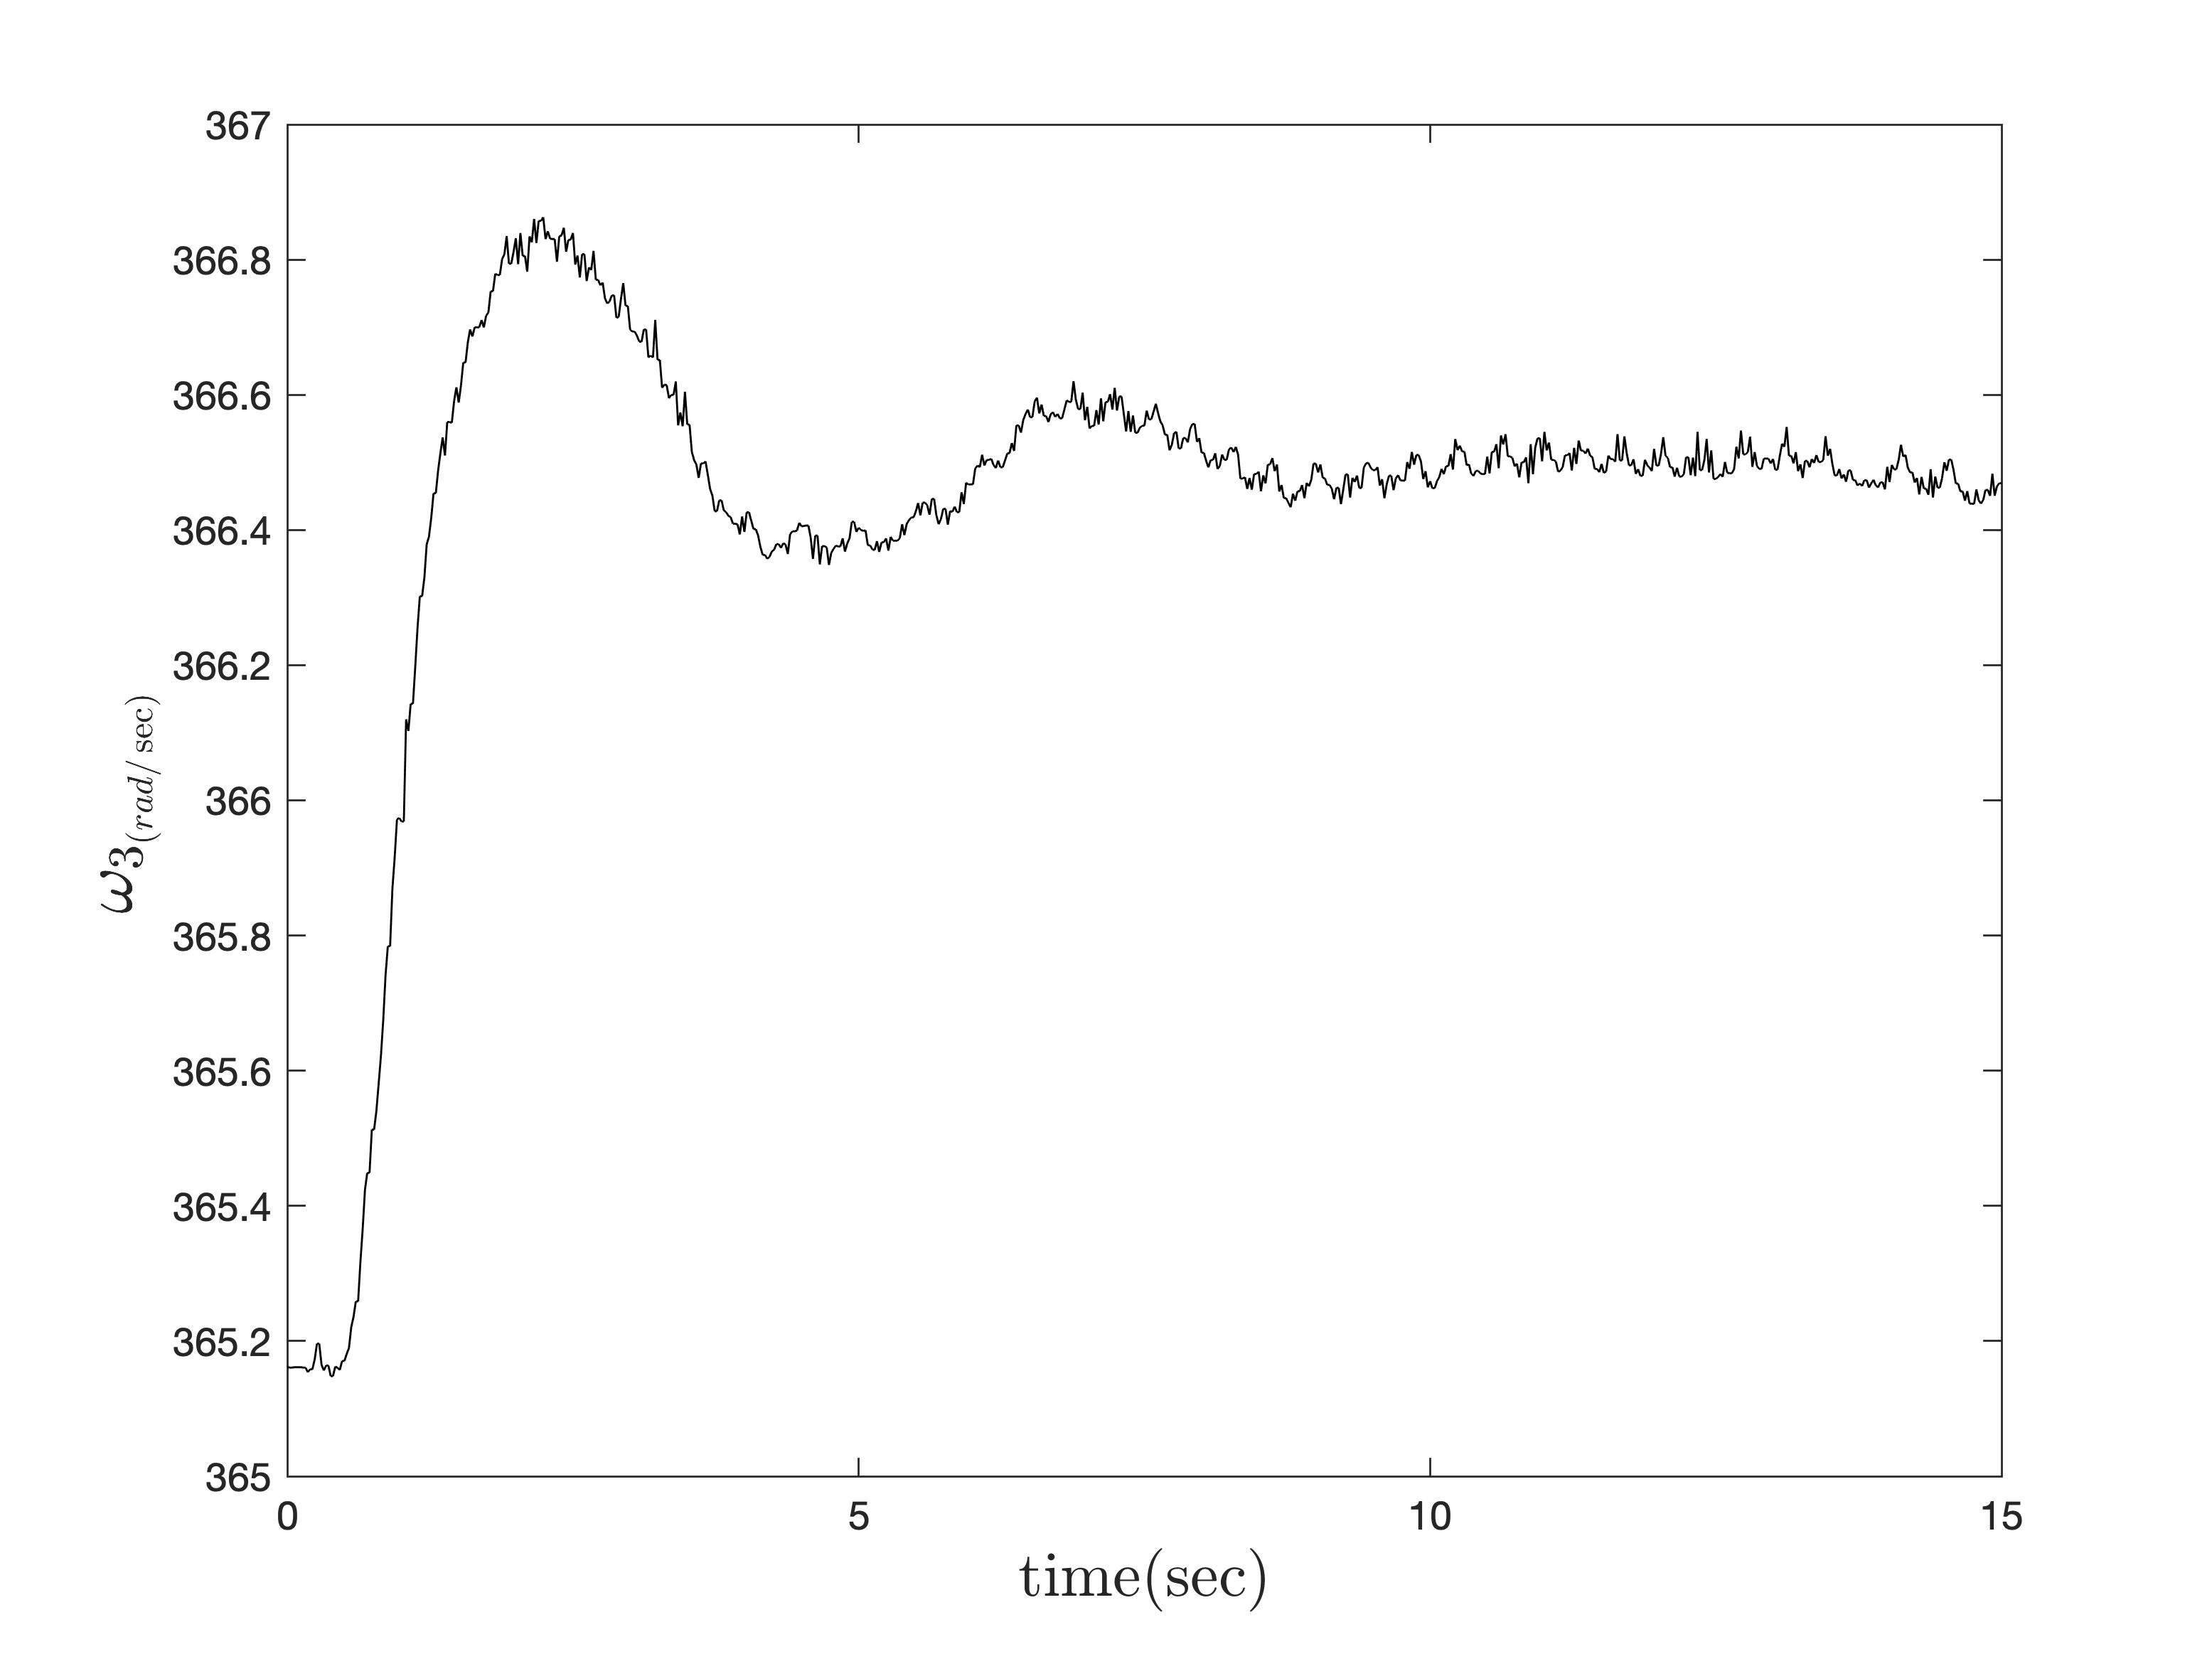
\includegraphics[width=12cm]{../Figures/Calibration/LQIDG/Pitch/lqidg_Omega_3.png}
%		\caption{موتور شماره سه}
%	\end{subfigure}
%	\caption{‫‪فرمان کنترل‌کننده موتور سه و چهار در کنترل زاویه رول و پیچ (تعقیب ورودی صفر)}
%\end{figure}

\begin{figure}[H]
	\centering
	\subfigure[موتور شماره یک]{
		\centering
		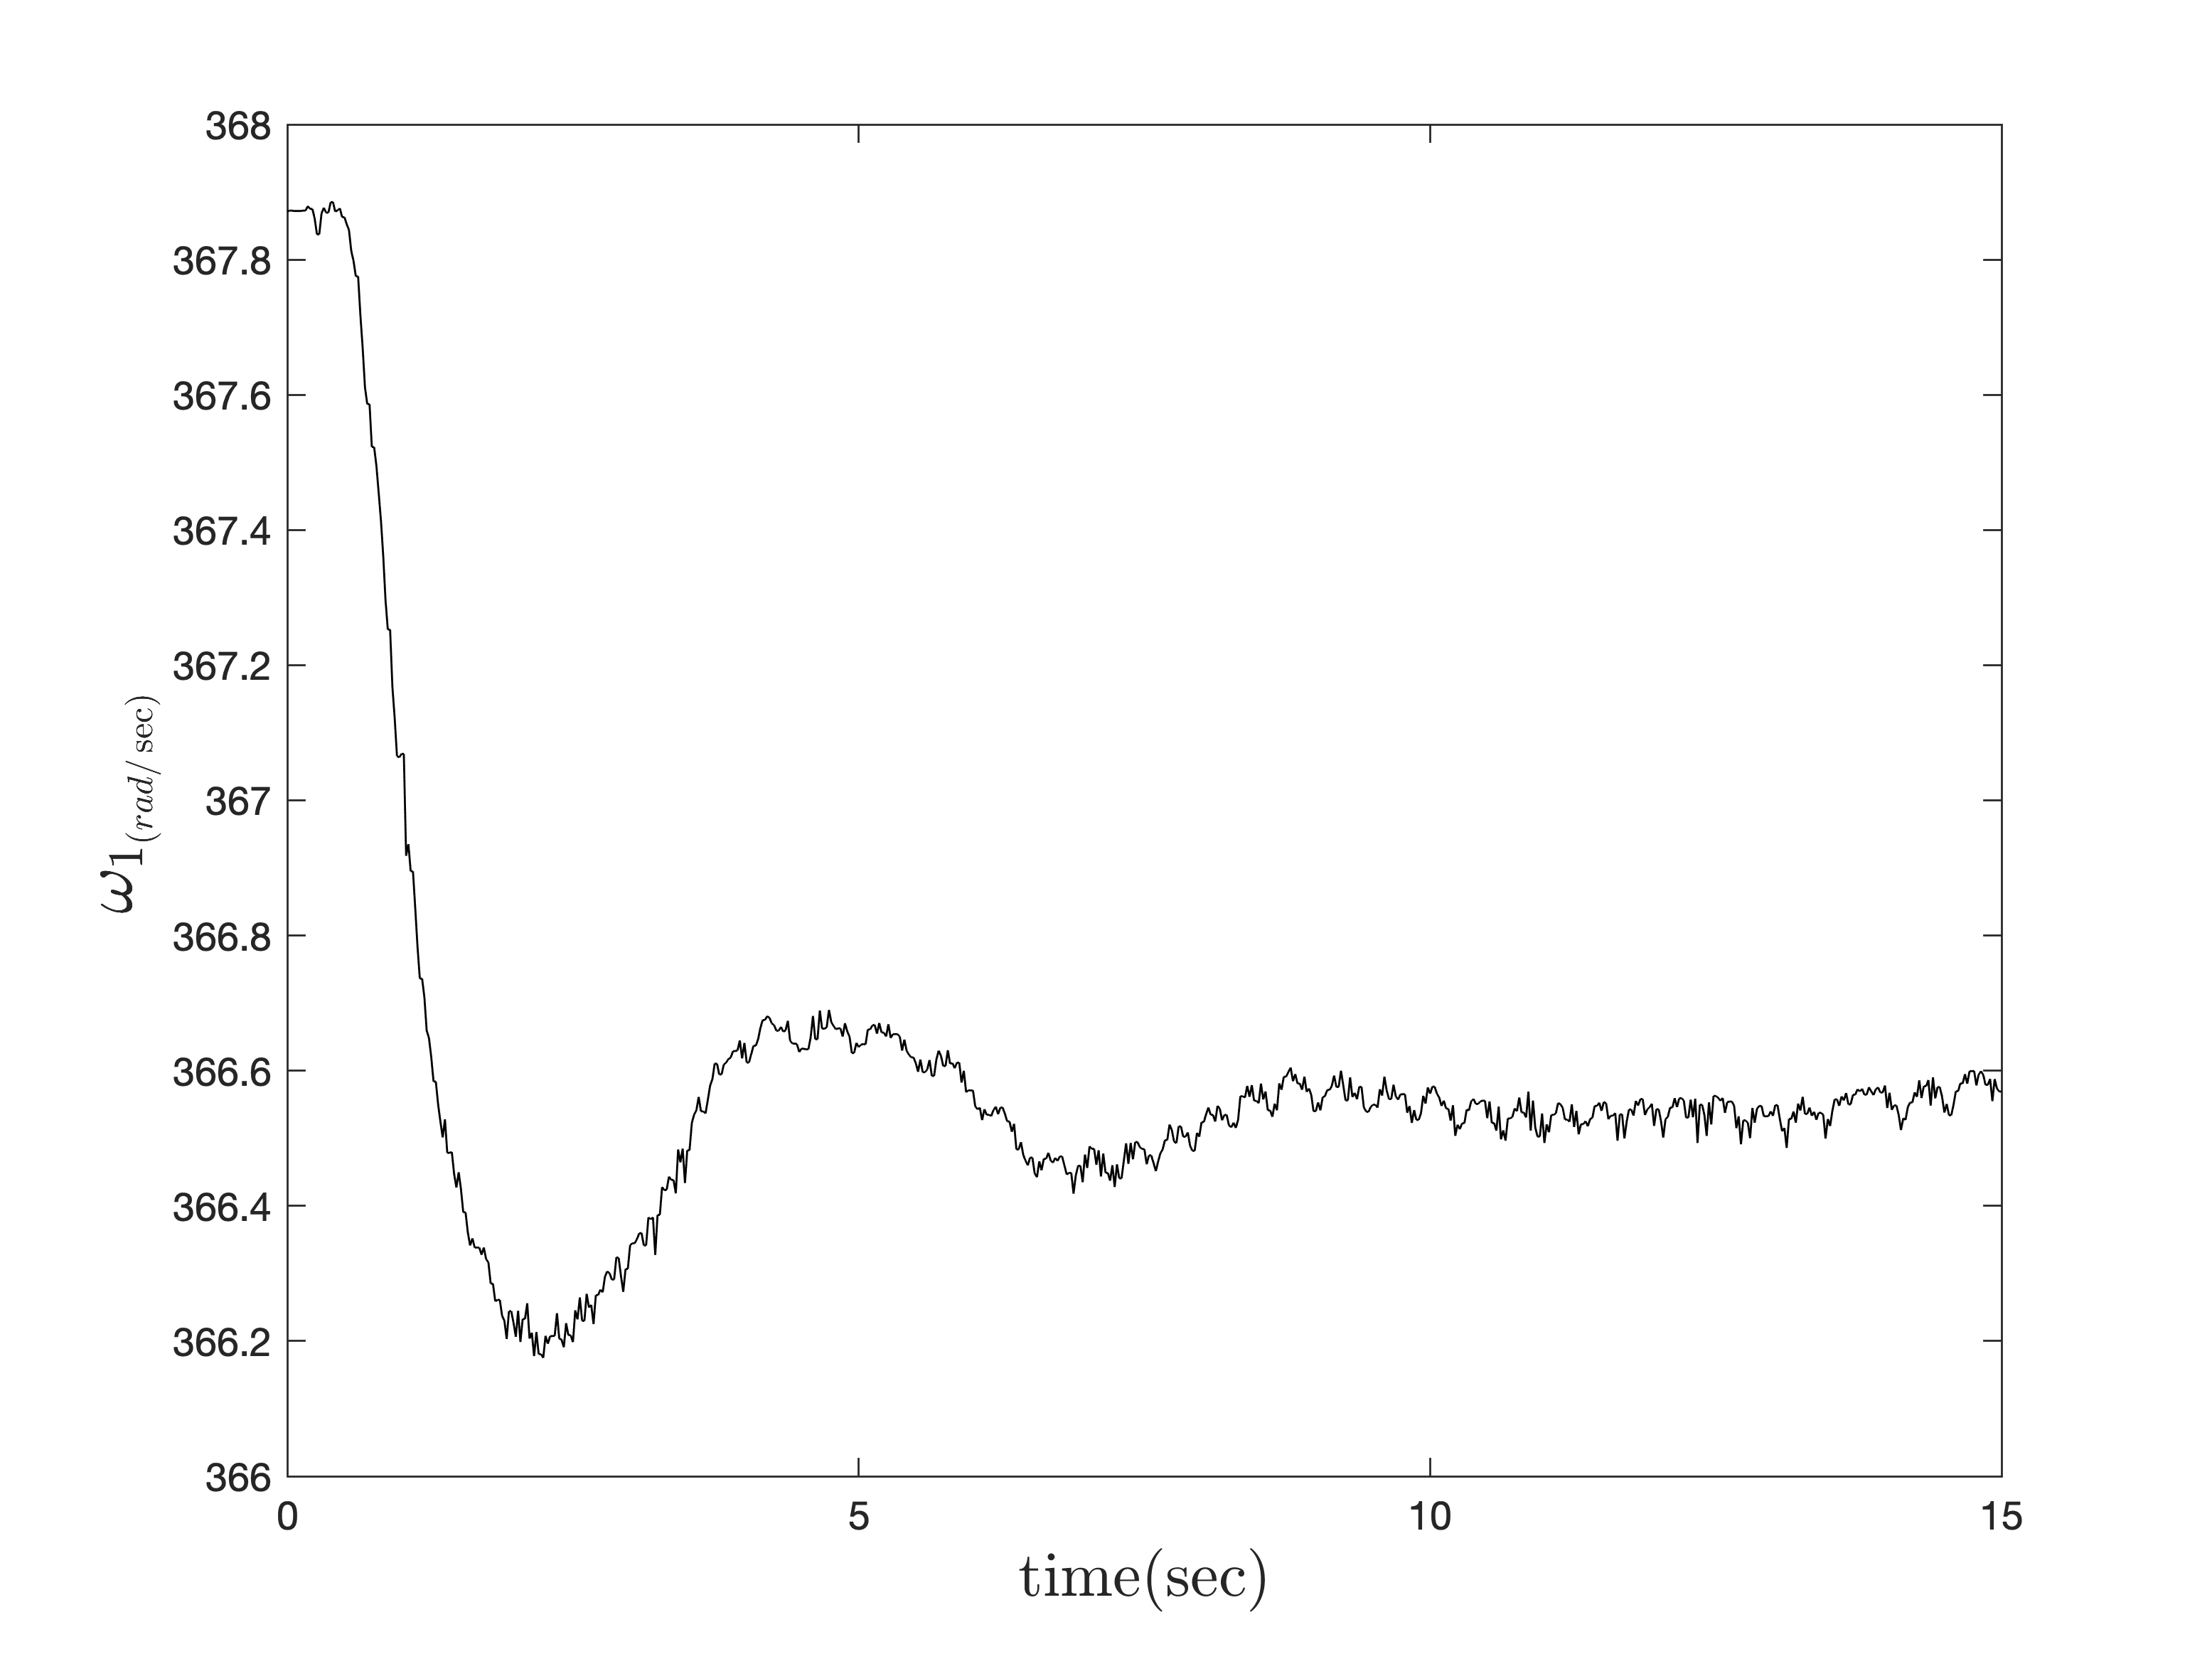
\includegraphics[width=.45\linewidth]{../Figures/Calibration/LQIDG/Pitch/lqidg_Omega_1.png}
	}
	\subfigure[موتور شماره سه]{
		\centering
		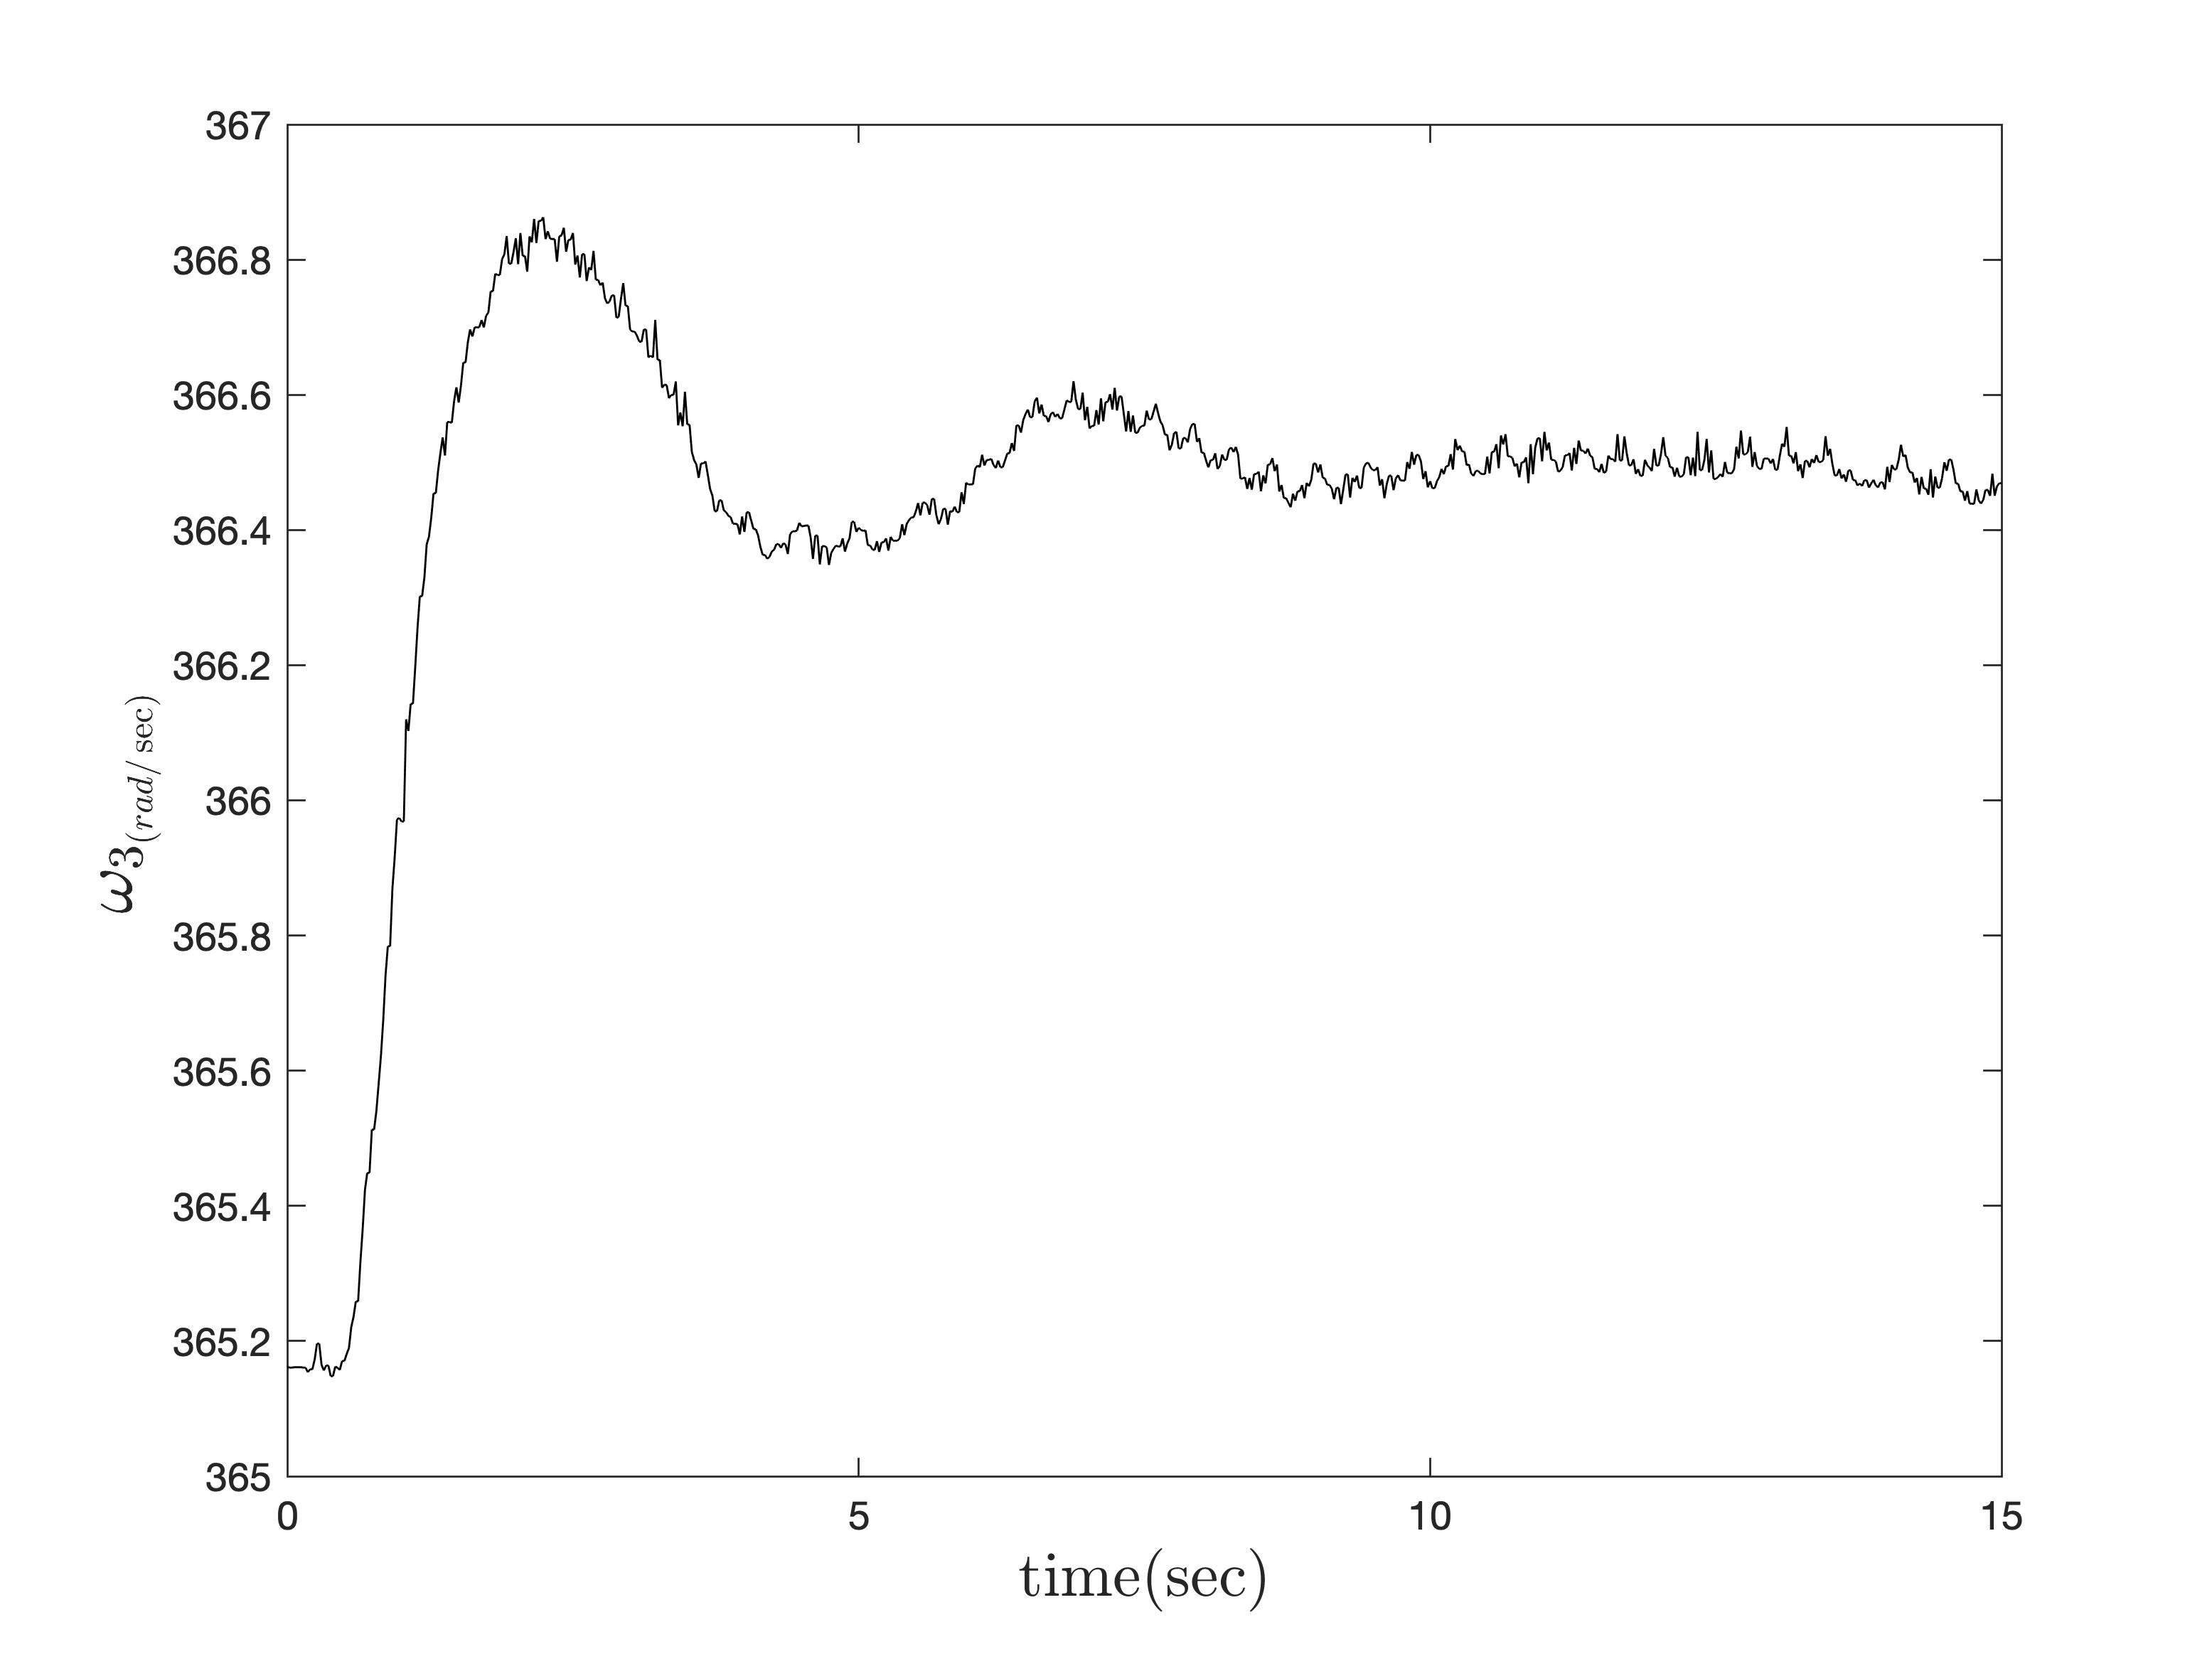
\includegraphics[width=.45\linewidth]{../Figures/Calibration/LQIDG/Pitch/lqidg_Omega_3.png}
	}
	
	\caption{‫‪فرمان کنترلی موتورهای یک و سه در کنترل زاویه پیچ (تعقیب ورودی صفر)}
\end{figure}



%بر اساس خروجی شبیه‌سازی (شکل
%\ref{lqidg_roll_fig})
%،کانال رول در حضور کنترل‌کننده LQIDG در حدود پنج ثانیه به تعادل می‌رسد و خطای ماندگار آن در حدود صفر است.